\documentclass{article}
\usepackage[utf8]{inputenc}
\usepackage[sc]{mathpazo}
\usepackage{graphicx}
\usepackage{url}
\usepackage{hyperref}
\usepackage{subcaption}
\usepackage{svg}

\graphicspath{ {./images/} }

\title{Preventing Secondary Structure Formation in the ADS Codex}
\author{Alina Li}
\date{Aug 5, 2022}

\begin{document} 
\maketitle

\begin{abstract}
In the field of bioinformatics, the formation of secondary structures increases the likelihood of DNA sequencing errors. In this paper, we explore how to prevent secondary structure formation in the context of DNA data storage. We contribute to the ADS codex, an open-source DNA codec, by integrating nucleic acid structure analysis to reduce the number of sequences with prominent secondary structures. We use random seeds and data randomization to produce variation in secondary structure prevalence, and found that the effect was minimal. We discuss next steps for secondary structure prevention in the codec.
\end{abstract}

\section{Introduction}
DNA data storage is an exciting field of research because it could reduce the need for traditional physical media in the coming decades. In the future, our digital data could be stored in DNA rather than hard drives, which has a number of advantages. First, DNA has high data density, in part due to the small and condensed nature of the molecule [1]. In 2017, for instance, researchers at Columbia University were able to encode 215 petabytes of data in a gram of DNA [6]. That data density could reach even higher values as technology advances. In addition to high data density, DNA data storage is also very scalable. Hardware changes over time whereas DNA remains the same -- a biological molecule that relies on common chemical processes for synthesis and sequencing [1].  

However, various obstacles prevent its adoption, including high costs and sequencing and synthesis errors [1]. Sequencing is the process of determining the order of nucleotides in DNA, and the cost has been steadily decreasing over the past two decades [5]. In addition to high costs, high error rates necessitate new methods avoiding and fixing error specific to DNA. Insertion, deletion, and substitution errors are some examples [1]. DNA codecs must be able to work around or fix these errors, or else fail to fully recover data. Currently, the ADS codex addresses errors resulting from a higher content of C and G nucleotides (two of the four possible DNA bases) and errors caused by homopolymers (repeating nucleotide sections). The codec uses  criteria that excludes long homopolymers to build encoding lookup tables. Then, using the lookup table, data is converted into nucleotide sequences. These nucleotide sequences are later checked for high GC content. If the GC content is greater than 60 percent, the complement of the sequence is taken. These two error prevention measures occur during the encoding phase, and as a second layer, errors are fixed during the decoding phase using alignment mechanisms and error correction codes. The codec currently does not account for errors resulting from secondary structures [1].

As a result, by addressing secondary structures in the ADS codex, we may contribute to fewer sequencing errors and greater data recovery. In the following sections, we give background on the software package NUPACK, which contains functionality for performing secondary structure analysis. We also describe how NUPACK has and could be integrated into the ADS codex in the future. Finally, we outline areas where further research is needed.

\section{DNA Analysis}
DNA, a two-stranded molecule, has a helical secondary structure, where the two strands' base pairs complement each other. For the purposes of this paper, DNA should not be considered in its double-stranded form, but rather as single strands, also known as oligos. These oligos are composed of sequences of four different nucleotides -- adenine, cytosine, guanine, and thymine. Beyond the sequence, oligos can form secondary structures. Secondary structures are defined by a strand's base pair interactions, where complementary sections of the strand can connect to each other, forming structures such as hairpin loops, stacking pairs, and others. 

\begin{figure}[!h]
\centering
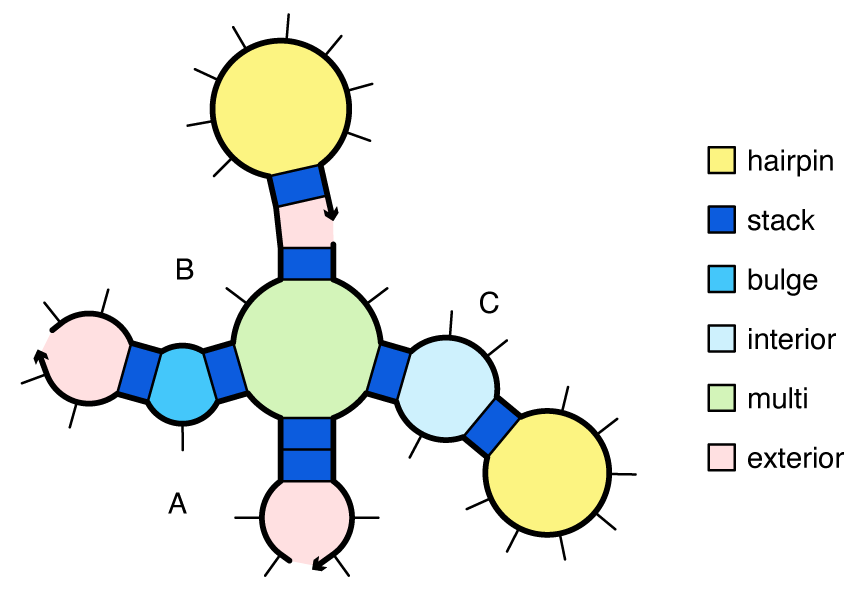
\includegraphics[scale=1]{secondary_structures_overview.png}
\caption{Examples of secondary structures from \url{https://docs.nupack.org/definitions}}   
\end{figure} 


Generally speaking, a given strand has the ability to form multiple different secondary structures. [2] Some structures are more prominent than others (ie. due to number and strength of bonds), meaning that they are more likely to interfere with sequencing. Quantitatively, we can compare secondary structures by calculating their free energy, a measure based on base pair interactions. Higher, Free energy measures the ability for a system to change, and in this case, it measures the change in energy from the unfolded state with no interactions to the secondary structure state. Larger, more negative values mean that the structure is more prominent. [Citation?] In Figure 2, two secondary structures with different free energies are shown. The DNA strand is the curve with nucleotides present at regular intervals. Some nucleotides are bonded to others, indicated by the short perpendicular lines. In Figure 2a, many of the bonds connecting complementary sections of the DNA strand are dark red, indicating high equilibrium probability (the probability of remaining in that state). A significant portion of the p     

\begin{figure}[!h]
\centering
\begin{subfigure}{.5\textwidth}
  \centering
  \includesvg[scale=.5]{mfe_low.svg}
  \caption{Large negative free energy}
  \label{fig:sub1}
\end{subfigure}%
\begin{subfigure}{.5\textwidth}
  \centering
  \includesvg[scale=.5]{mfe_high.svg}
  \caption{Small negative free energy}
  \label{fig:sub2}
\end{subfigure}
\caption{Secondary structures with different free energies. Images generated by NUPACK}
\label{fig:test}
\end{figure}

NUPACK, a software package, conveniently provides a variety of commands for analyzing nucleotide sequences, including probability of structure formation, free energy of a structure, and minimum free energy. [give background on free energy] For determining which strands will form the most prominent secondary structures, the minimum free energy is a valuable metric. The larger and more negative the free energy for a given secondary structure is, the more stable that structure is, and the more likely it is to interfere with synthesis and sequencing processes. [explain why it might interfere? do a little more research about this] The ADS codex produces a set of DNA strands based on an input file. Running the MFE (minimum free energy) calculation on each strand can help determine the likelihood of prominent secondary structure formations.

One heuristic for determining which oligos have structures that will interfere with sequencing is physics-based. A given strand can either be in the folded or extended state. Statistical mechanics [??] calculations applied to nucleotide sequences say that the free energy threshold between the folded and extended state is equal to $-ln(f_0) * k_B * T$, where $f_0$ is the fraction of folded molecules, $k_B$ is Boltzmann’s constant (a constant in [some field of study]), and T is the temperature of the strands. After running MFE calculations for each strand, one may be able to determine the fraction of oligos that are folded and therefore difficult to sequence. An alternative heuristic relies on data from previous experiments. [4]

\section{Integration}

For the ADS codex, our goal is to encode the data in such a way that reduces the effect of prominent secondary structures in the encoded data. If data is encoded into DNA strands that have prominent secondary structures which end up increasing the sequencing and synthesis error rates, the data may be difficult to recover from the DNA strands. 

The ADS codex encoder uses a lookup table to encode data -- one sequence of bits corresponds to a specific sequence of nucleotides. Therefore, to find encodings with less secondary structures, we can randomize the data itself to produce different nucleotide sequences. Then, by comparing each set of oligos, one can choose the set with the fewest secondary structures. The codec already implements a randomization scheme by generating numbers from a PRNG and XORing those numbers with the original data. ??? for seeds 1-100, each seed produced an average of ? character changes excluding the 6-nt long primers at the beginning and ??. 

In the following section we will describe methods of choosing the “best” random seed for randomizing the data and producing the "best" encoding. 

For background, the ADS codex allows us to specify the random seed. The encoder returns a list of nucelotide sequences, which we then analyzed using NUPACK and its commands.

We began by comparing the average MFE of a given encoding. After running the DNA encoder, we ran the MFE calculation on each oligo and took the average. The idea here is to choose the random seed that produces the least negative MFE average.

\section{Results}
We generated a random 32k byte file and inputted the file into the ADS encoder, using the --rndseed flag to specify the seed for the PRNG, and subsequently, the data randomization. We tested random seeds 1, 10, 50, and 100. The encoder spit out a list of 2740 DNA sequences. We then ran MFE calculations on each sequence, and plotted the MFE values in a histogram and calculated the average MFE.

\includesvg[scale=0.5]{32k_default_histogram.svg}

The histograms indicate a common bell-curve trend despite data randomization. This indicates that randomizing the data will produce some oligos with high MFEs, some with low MFEs, and most oligos with an average MFE value of approximately -14 kcal/mol. The average MFE across the four data sets reflects this as well: the range is a mere 115 thousandths kcal/mol. Therefore, selecting the random seed via method 1 -- by simply comparing averages -- may not be particularly effective.


\section{Conclusion}
A more advanced approach could consider using the heuristics described above for determining the oligos most likely to form secondary structures. Since the encoder produces both erasure oligos and data oligos, one could analyze the disposability of certain oligos. 

Future research will refine the heuristic for determine the "bad" oligos, and develop a sound method for choosing a random seed. Laboratory tests will also help determine whether these analyses affect the error rates of the data storage process.

\section{Citations}
[refine this; actually do citations]

1 ADS codex paper 


2 MFE, secondary structures
Thermodynamic Analysis of
Interacting Nucleic Acid Strands 

3 nupack docs on secondary structures, loops, free energy calculations,
https://docs.nupack.org/ 
UserGuide PDF nupack 3.2.2

4 jason gans emails; heuristics

5 sequencing costs 
https://www.genome.gov/about-genomics/fact-sheets/DNA-Sequencing-Costs-Data

6 columbia university 1g of dna 
https://www.science.org/doi/full/10.1126/science.aaj2038



\end{document}